% Provenance (never printed): see sources/outline_sources.md (Year 1: compaction and
% cementation; basin types; subsidence, accommodation and sea-level change). Exercise and
% problem values in the Book 3 scratch calculator calc/ch23.py; figure data from
% figdata/bachelor-1/compaction.py and sea_level.py.
% Porosity and permeability are Book 1's (g6); diagenesis was met in Book 2 (g12) and is
% re-founded here; sedimentary basin was met in Book 2 (g11) and is re-founded here;
% isostasy and the equal-mass proposition are ch. 11's; passive margins and rifts ch. 13's;
% effective stress ch. 16's; the Last Glacial Maximum and glacial cycles Book 2's (g12).
% Pressure solution is defined in the Year 3 volume (deformation mechanisms): prose only.
% Backstripping, the stretching model and the comparison of basins are the Year 2 volume's.
\chapter{डायाजेनेसिस और अवसादी द्रोणियाँ}\label{ch:b1:diagenesis-basins}

समुद्र-तट की बालू ढीली है: उसके आयतन का आधा भाग कणों के बीच का पानी है। तीन किलोमीटर नीचे दबी वही बालू ड्रिल-कोर में कठोर बलुआ पत्थर बनकर ऊपर आती है, उसके कण एक-दूसरे पर दबे हुए, उनके बीच का स्थान बहुत कम हुआ और आंशिक रूप से नए क्वार्ट्ज से भरा हुआ। तट और कोर के बीच लाखों वर्ष हैं, जिनमें तलछट पर और तलछट जमी, उसे निचोड़ा गया, गरम किया गया, और ऐसे पानी में भिगोया गया जिसने कुछ \omterm{def:b1:rock-forming-minerals:mineral}{खनिज} घोले और दूसरे अवक्षेपित किए। यह अध्याय उन परिवर्तनों का अनुसरण करता है, फिर उन स्थानों की ओर लौटता है जहाँ तलछट किलोमीटरों मोटी ढेर हो सकती है --- अवसादी द्रोणियाँ --- और उन दो चीज़ों की ओर जो वहाँ उसके लिए जगह बनाती हैं: फ़र्श का धँसना, और समुद्र का उठना और गिरना।

\begin{recall}
किसी चट्टान की छिद्रता उसके आयतन का वह भाग है जो छिद्रों से बना है, और उसकी पारगम्यता मापती है कि पानी उनमें से कितनी आसानी से बहता है (पुस्तक~1, कक्षा~6)। एक क्षेत्र समस्थितिक तब होता है जब संतुलन-गहराई तक हर स्तंभ में वही द्रव्यमान हो (\cref{prop:b1:isostasy-gravity:equal-mass})। दरारें सामान्य भ्रंशन से खुलती हैं, और निष्क्रिय किनारे महाद्वीपों के वे किनारे हैं जो तब बचते हैं जब एक दरार महासागर बन जाती है (\cref{ch:b1:rifts-ridges-margins})। \omterm{def:b1:stress-strain-rheology:lithostatic}{प्रभावी प्रतिबल} वह प्रतिबल है जिसमें से \omterm{def:b1:stress-strain-rheology:lithostatic}{छिद्र-द्रव दाब} घटा हो (\cref{def:b1:stress-strain-rheology:lithostatic})। अंतिम हिमनद चक्र लगभग बीस हज़ार वर्ष पहले अपने अंतिम हिमनद उच्चिष्ठ पर पहुँचा (पुस्तक~2, कक्षा~12)। बलुआ पत्थर, शेल और उनके परिवेश \cref{ch:b1:clastic-sediments} के हैं; चूना-पत्थर, चॉक, डोलोमाइट और \omterm{def:b1:chemical-biogenic-sediments:evaporite}{वाष्पनिक निक्षेप} \cref{ch:b1:chemical-biogenic-sediments} के।
\end{recall}

\section{संपीड़न}\label{sec:b1:diagenesis-basins:compaction}

नया जमा तलछट कणों का एक ढीला संग्रह है, जिनके बीच पानी है। निक्षेपण के बाद और रूपांतरण से पहले उसके साथ जो कुछ होता है, जब तक वह पृथ्वी की पपड़ी के ऊपरी कुछ किलोमीटर के निम्न तापमान और दाब पर रहता है, वह एक ही परिवार की प्रक्रियाओं से संबंधित है।

\begin{definition}[डायाजेनेसिस]\label{def:b1:diagenesis-basins:diagenesis}
\emph{डायाजेनेसिस}\index{डायाजेनेसिस} वे भौतिक, रासायनिक और जैविक परिवर्तन हैं जो एक तलछट अपने निक्षेपण के बाद पाती है, पृथ्वी की ऊपरी पपड़ी के तापमान और दाब पर, रूपांतरण के दाब और तापमान से नीचे। इसमें \omterm{def:b1:diagenesis-basins:compaction}{संपीड़न}, \omterm{def:b1:diagenesis-basins:cement}{सीमेंटन}, कणों का घुलना, और एक \omterm{def:b1:rock-forming-minerals:mineral}{खनिज} का दूसरे से प्रतिस्थापन शामिल हैं; ये मिलकर एक ढीले तलछट को अवसादी शैल में बदलते हैं।
\end{definition}

इन परिवर्तनों में पहला यांत्रिक है। हर नई परत अपना भार नीचे की परतों पर डालती है। कण एक-दूसरे पर दबते हैं, सरकते और घूमते हैं एक कसे हुए विन्यास में, नरम कण (मृत्तिका के पत्र, शैल-टुकड़े, \omterm{def:b1:rock-forming-minerals:groups}{अभ्रक}) कठोर कणों के बीच मुड़ जाते हैं, और उनके बीच का पानी बाहर निकल जाता है।
% ledger: og:diagenesis

\begin{definition}[संपीड़न, डिकंपैक्शन]\label{def:b1:diagenesis-basins:compaction}
\emph{संपीड़न}\index{संपीड़न} ऊपर के तलछटों के भार के नीचे एक तलछट के आयतन की हानि है, उसके कणों की निकट पैकिंग से, उसके छिद्र-जल के निष्कासन से, और गहराई पर, उन स्थानों पर कणों के घुलने से जहाँ वे एक-दूसरे को छूते हैं। \emph{डिकंपैक्शन}\index{डिकंपैक्शन} वह गणना है जो एक दबी परत को उस मोटाई पर लौटाती है जो उसकी किसी पूर्व, उथली दबी अवस्था में थी, प्रायः सतह पर, जब वह जमी थी।
\end{definition}

कुओं में मापी गई छिद्रताएँ गहराई के साथ घटती हैं, सतह के पास तीव्रता से और फिर अधिकाधिक धीरे-धीरे। 1930 में एथी ने उन्हें एक घातांक से समायोजित किया, और तब से वह समायोजन \omterm{def:b1:diagenesis-basins:compaction}{संपीड़न} अध्ययनों का आरंभ-बिंदु रहा है।
% ledger: sc80:athy

\begin{proposition}[एथी का नियम]\label{prop:b1:diagenesis-basins:athy}
एक ही शैल-प्रकार के तलछट के ढेर में, जो अपने भार के नीचे संपीड़ित होता है और जिसका छिद्र-जल निकलने के लिए स्वतंत्र है, सतह के नीचे गहराई $z$ पर छिद्रता
\[
  \varphi(z) = \varphi_0\, e^{-z/\lambda},
\]
जहाँ $\varphi_0$, सतही छिद्रता, और $\lambda$, क्षय-लंबाई, शैल-प्रकार पर निर्भर करते हैं। यह \emph{एथी का नियम}\index{एथी का नियम} है।
\end{proposition}
\admitted

नियम एक अनुभवजन्य समायोजन है, सिद्धांत का परिणाम नहीं। उसके प्राचल हर शैल-प्रकार के लिए कुओं की छिद्रताओं से मापे जाते हैं; \cref{tab:b1:diagenesis-basins:athy} के मान, जो उत्तरी सागर के \omterm{def:b1:diagenesis-basins:subsidence}{अवधसान} के एक अध्ययन के साथ प्रकाशित हुए, \omterm{def:b1:diagenesis-basins:compaction}{संपीड़न} के लिए सुधार करने में व्यापक रूप से उपयोग होते हैं। शेल अधिक पानी लेकर शुरू करता है पर उसे कम दूरी में खोता है; चॉक, जो सतह पर तीनों में सबसे अधिक छिद्रमय है, उसे सबसे तेज़ी से खोता है। \qty{3000}{m} पर नियम बलुआ पत्थर के लिए \num{0.22}, शेल के लिए \num{0.14} और चॉक के लिए \num{0.08} छिद्रता देता है (नीचे का चित्र): आरंभिक अनुच्छेद की समुद्र-तट बालू ने अपने छिद्रों का आधे से अधिक खो दिया है।
% ledger: pybacktrack:compaction, sc80:north-sea

\begin{table}[htbp]
\centering
\begin{tabular}{lccc}
\hline
शैल-प्रकार & सतही छिद्रता $\varphi_0$ & क्षय-लंबाई $\lambda$ (m) & कणों का घनत्व (\unit{kg.m^{-3}}) \\
\hline
शेल            & 0.63 & 1960 & 2700 \\
बलुआ पत्थर        & 0.49 & 3704 & 2650 \\
शेलीय बलुआ पत्थर  & 0.56 & 2564 & 2680 \\
चॉक            & 0.70 & 1408 & 2710 \\
\hline
\end{tabular}
\caption{एथी के नियम के प्राचल और चार शैल-प्रकारों के कणों के घनत्व, स्क्लेटर और क्रिस्टी (1980) के अनुसार, जैसा खुले बैकट्रैकिंग सॉफ़्टवेयर पाइबैकट्रैक में सारणीबद्ध है।}
\label{tab:b1:diagenesis-basins:athy}
\end{table}
% ledger: pybacktrack:compaction

\omterm{def:b1:diagenesis-basins:compaction}{संपीड़न} पानी निचोड़ता है; वह न कण जोड़ता है न हटाता है, जब तक कुछ घुलकर बाहर न ले जाया जाए या \omterm{def:b1:diagenesis-basins:cement}{सीमेंट} के रूप में भीतर न लाया जाए। स्तंभ के कणों का आयतन इसलिए वही मात्रा है जिसे स्तंभ के दबने के साथ अनुसरण करना है।

\begin{proposition}[परत की ठोस मोटाई]\label{prop:b1:diagenesis-basins:solid}
एथी के नियम के अंतर्गत, गहराइयों $z_1 < z_2$ के बीच की एक परत प्रति इकाई क्षेत्रफल में कणों का वह आयतन रखती है जो इस मोटाई के बराबर है
\[
  s = (z_2 - z_1) - \varphi_0 \lambda \left( e^{-z_1/\lambda} - e^{-z_2/\lambda} \right).
\]
यदि परत बिना कणों की हानि या लाभ के एक नई गहराई पर ले जाई जाए, तो उसके नए ऊपरी $z_1'$ और निचले $z_2'$ संतुष्ट करते हैं $s(z_1', z_2') = s(z_1, z_2)$, और दिए गए
$z_1'$ के लिए इस समीकरण का ठीक एक हल $z_2'$ है।
\end{proposition}

\begin{proof}
मोटाई $\mathrm dz$ की एक परत, गहराई $z$ पर, प्रति इकाई क्षेत्रफल में कणों का आयतन $(1 - \varphi(z))\,\mathrm dz$ रखती है। $z_1$ से $z_2$ तक समाकलित करने पर,
\[
  s = \int_{z_1}^{z_2} \bigl(1 - \varphi_0 e^{-z/\lambda}\bigr)\,\mathrm dz
    = (z_2 - z_1) - \varphi_0\lambda\left(e^{-z_1/\lambda} - e^{-z_2/\lambda}\right).
\]
$z_1'$ पर स्थिर ऊपरी सतह के साथ, फलन $f(b) = s(z_1', b)$ का अवकलज $1 - \varphi(b) > 0$ है, क्योंकि छिद्रता एक से कम है; वह सतत है, $b = z_1'$ पर शून्य है और बिना सीमा के बढ़ता है, इसलिए वह मान $s(z_1, z_2)$ ठीक एक बार लेता है।
\end{proof}

\begin{method}[एक परत का डिकंपैक्शन]\label{met:b1:diagenesis-basins:decompaction}
\begin{enumerate}
  \item आज परत का ऊपरी $z_1$ और निचला $z_2$ पढ़िए, और उसके प्राचल $\varphi_0$ और $\lambda$
        (\cref{tab:b1:diagenesis-basins:athy})।
  \item \cref{prop:b1:diagenesis-basins:solid} से उसकी ठोस मोटाई $s$ परिकलित कीजिए।
  \item उसके ऊपरी $z_1'$ की वह गहराई चुनिए जो पहले के समय में थी --- उसे सतह पर लौटाने के लिए शून्य।
  \item $s(z_1', b) = s$ को नए निचले $b$ के लिए न्यूटन की विधि से हल कीजिए:
        $b_0 = z_1' + (z_2 - z_1)$ से आरंभ कीजिए और दोहराइए
        \[
          b_{k+1} = b_k - \frac{s(z_1', b_k) - s}{1 - \varphi(b_k)}
        \]
        जब तक परिवर्तन वांछित परिशुद्धता से नीचे न हो जाए; आम तौर पर दो या तीन चरण पर्याप्त होते हैं।
  \item परत की उस समय की मोटाई $b - z_1'$ है; उसकी औसत छिद्रता $1 - s/(b - z_1')$ है।
\end{enumerate}
\end{method}

\qty{3000}{m} और \qty{3500}{m} के बीच \qty{500}{m} शेल लीजिए। उसमें \qty{440}{m} कण और केवल \qty{60}{m} पानी है, औसत छिद्रता \num{0.12}। सतह पर लाए जाने पर वही कण \qty{891}{m} मोटी परत बनाते हैं, जिसका आधा पानी है (नीचे का चित्र)। दबे हुए शेल की मोटाई जितनी जमी थी उसके बमुश्किल आधे से कुछ अधिक है; दबे हुए परिच्छेदों से पढ़ी गई तलछट-दरों की तुलना आज मापी गई दरों से करने से पहले उनका \omterm{def:b1:diagenesis-basins:compaction}{डिकंपैक्शन} करना होगा।
% computed in figdata/bachelor-1/compaction.py; ledger: pybacktrack:compaction

\begin{omfigure}
\begin{tikzpicture}[font=\footnotesize]
\begin{axis}[name=phi, width=7.6cm, height=7.2cm, xmin=0, xmax=0.75, ymin=0, ymax=5000,
    y dir=reverse, xlabel={छिद्रता $\varphi$}, ylabel={गहराई (m)},
    xtick={0,0.2,0.4,0.6}, ytick={0,1000,...,5000},
    legend style={at={(0.97,0.03)}, anchor=south east, font=\scriptsize, draw=none, fill=white, fill opacity=0.85, text opacity=1},
    legend cell align=left]
  \addplot[thick, omLithSand!50!black] table[x=phi_sand, y=z] {figdata/out/bachelor-1-compaction-curves.dat};
  \addplot[thick, omThm, densely dashed] table[x=phi_shale, y=z] {figdata/out/bachelor-1-compaction-curves.dat};
  \addplot[thick, omLithLime!50!black, dash dot] table[x=phi_chalk, y=z] {figdata/out/bachelor-1-compaction-curves.dat};
  \legend{बलुआ पत्थर, शेल, चॉक}
  \draw[black!50, dotted] (axis cs:0,3000) -- (axis cs:0.75,3000);
\end{axis}
\begin{axis}[at={(phi.east)}, anchor=west, xshift=1.6cm, width=6.4cm, height=7.2cm,
    ybar stacked, bar width=1.1cm, ymin=0, ymax=1000, enlarge x limits=0.45,
    symbolic x coords={buried, surface}, xtick=data,
    xticklabels={{3000--3500 m पर}, {सतह पर}},
    ylabel={परत की मोटाई (m)}, ytick={0,200,...,1000},
    legend style={at={(0.03,0.97)}, anchor=north west, font=\scriptsize, draw=none},
    legend cell align=left]
  \addplot[fill=omLithShale, draw=black!60] table[x=state, y=solid] {figdata/out/bachelor-1-compaction-demo.dat};
  \addplot[fill=omSea, draw=black!60] table[x=state, y=pore] {figdata/out/bachelor-1-compaction-demo.dat};
  \legend{कण, छिद्र-जल}
  \node[anchor=south] at (axis cs:buried,500) {\qty{500}{m}};
  \node[anchor=south] at (axis cs:surface,891) {\qty{891}{m}};
\end{axis}
\end{tikzpicture}

{\small बाईं ओर: एथी के नियम से गहराई के विरुद्ध बलुआ पत्थर, शेल और चॉक की छिद्रता, \cref{tab:b1:diagenesis-basins:athy} के प्राचलों के साथ। दाईं ओर: \qty{3000}{m} और \qty{3500}{m} के बीच \qty{500}{m} शेल, और वही परत सतह तक डिकंपैक्ट की गई: कण (\qty{440}{m}) बचे हैं, पानी नहीं।}
\label{fig:b1:diagenesis-basins:compaction}
\end{omfigure}
% computed in figdata/bachelor-1/compaction.py; ledger: pybacktrack:compaction

\omterm{prop:b1:diagenesis-basins:athy}{एथी का नियम} तभी लागू होता है जब तक पानी निकल सकता है। \omterm{def:b1:diagenesis-basins:compaction}{संपीड़न} \omterm{def:b1:stress-strain-rheology:lithostatic}{प्रभावी प्रतिबल} से चलता है, यानी ऊपर की चट्टान का भार घटा छिद्रों के पानी का दाब (\cref{ch:b1:stress-strain-rheology})। जहाँ एक मोटा शेल इतनी तेज़ी से दबता है कि उसका पानी रिसकर नहीं निकल सकता, वहाँ पानी भार का एक भाग उठाता है, छिद्र-दाब जल-स्थैतिक से ऊपर उठता है, और शेल अपनी गहराई के लिए बहुत अधिक छिद्रता रखता है: वह अतिदाबित है, और \omterm{def:b1:diagenesis-basins:compaction}{संपीड़न} के लिए सुधार को इसका हिसाब रखना होगा।
% ledger: sc80:north-sea

गहराई पर \omterm{def:b1:diagenesis-basins:compaction}{संपीड़न} रासायनिक बन जाता है। जहाँ दो क्वार्ट्ज कण पानी की एक परत के माध्यम से एक-दूसरे पर दबते हैं, और विशेषकर जहाँ मृत्तिका या \omterm{def:b1:rock-forming-minerals:groups}{अभ्रक} का एक पत्र उनके बीच है, वहाँ \omterm{def:b1:geological-maps:geological-map}{संपर्क} पर क्वार्ट्ज घुलता है; सिलिका पानी के माध्यम से थोड़ी दूरी तक विसरित होती है और खुले छिद्रों की ओर मुख किए स्वच्छ क्वार्ट्ज सतहों पर पुनः जमा हो जाती है। कण एक-दूसरे में अंतर्गुंफित हो जाते हैं, और सतहों के साथ केंद्रित घुलना स्टाइलोलाइट छोड़ता है, अघुलनशील अवशेष की दाँतेदार सीवनें। यह दाब-विलयन, जिसे पुस्तक~5 में विरूपण की एक यंत्रणा के रूप में लिया गया है, \omterm{def:b1:diagenesis-basins:compaction}{संपीड़न} की अंतिम अवस्था भी है और बलुआ पत्थरों के सबसे आम \omterm{def:b1:diagenesis-basins:cement}{सीमेंट} का स्रोत भी।
% ledger: walderhaug:quartz, oye:quartz-cement

\section{सीमेंटन और अन्य परिवर्तन}\label{sec:b1:diagenesis-basins:cementation}

\omterm{def:b1:diagenesis-basins:compaction}{संपीड़न} अकेला एक सघन तलछट बनाता है, कठोर शैल नहीं। कणों को उन खनिजों द्वारा एक शैल में चिपकाया जाता है जो छिद्रों में उगते हैं।

\begin{definition}[सीमेंटन, सीमेंट]\label{def:b1:diagenesis-basins:cement}
\emph{सीमेंटन}\index{सीमेंटन} तलछट के छिद्रों में, छिद्र-जल से खनिजों का अवक्षेपण है, जो उसके कणों को एक-दूसरे से बाँधता है और उसकी छिद्रता घटाता है। इस प्रकार अवक्षेपित \omterm{def:b1:rock-forming-minerals:mineral}{खनिज} शैल का \emph{सीमेंट}\index{सीमेंट} बनाते हैं; सबसे आम हैं क्वार्ट्ज, कैल्साइट, लौह ऑक्साइड और \omterm{def:b1:weathering-clays:clay-mineral}{मृत्तिका-खनिज}।
\end{definition}

भूजल \omterm{def:b1:diagenesis-basins:cement}{सीमेंट} करने वाले खनिजों को घोल में ले जाता है, और वे कणों के संघटन के समान होने ज़रूरी नहीं। लौह ऑक्साइड कणों पर परत चढ़ाते हैं और चट्टानों को लाल, भूरा या पीला रंग देते हैं, जैसे कोलोराडो पठार की परतों में; कैल्साइट बलुआ पत्थरों और चूना-पत्थरों दोनों को \omterm{def:b1:diagenesis-basins:cement}{सीमेंट} करता है।
% ledger: og:diagenesis

क्वार्ट्ज गहराई में दबे बलुआ पत्थरों का \omterm{def:b1:diagenesis-basins:cement}{सीमेंट} है। वह मूल क्वार्ट्ज कणों पर उनके साथ प्रकाशीय निरंतरता में, अतिवृद्धियों के रूप में उगता है: सूक्ष्मदर्शी में, क्रॉस्ड पोलराइज़रों के बीच, एक कण और उसकी अतिवृद्धि एक साथ काले पड़ते हैं, और कण की मूल रूपरेखा केवल धूल या मृत्तिका की एक पतली कोर के रूप में दिखती है (नीचे का चित्र)। उत्तरी सागर और टेक्सस के बलुआ पत्थरों में, जिनका विस्तार से अध्ययन हुआ है, अतिवृद्धियों के ऑक्सीजन समस्थानिक दिखाते हैं कि \omterm{def:b1:diagenesis-basins:cement}{सीमेंट} \qtyrange{60}{80}{\celsius} पर उगना शुरू हुआ और चट्टानों के अधिकतम दफ़न-तापमान तक चलता रहा; टेक्सस के बलुआ पत्थरों में \qtyrange{12}{18}{\percent} क्वार्ट्ज \omterm{def:b1:diagenesis-basins:cement}{सीमेंट} है, उत्तरी सागर वालों में केवल \qtyrange{2}{6}{\percent}, और अधिकांश सिलिका कण-संपर्कों पर दाब-विलयन से आई। क्योंकि क्वार्ट्ज केवल स्वच्छ क्वार्ट्ज सतहों पर उगता है, कणों पर मृत्तिका की एक परत \omterm{def:b1:diagenesis-basins:cement}{सीमेंट} के लिए कम सतह छोड़ती है और एक गहरे बलुआ पत्थर की छिद्रता बचा सकती है।
% ledger: oye:quartz-cement, walderhaug:quartz

\begin{omfigure}
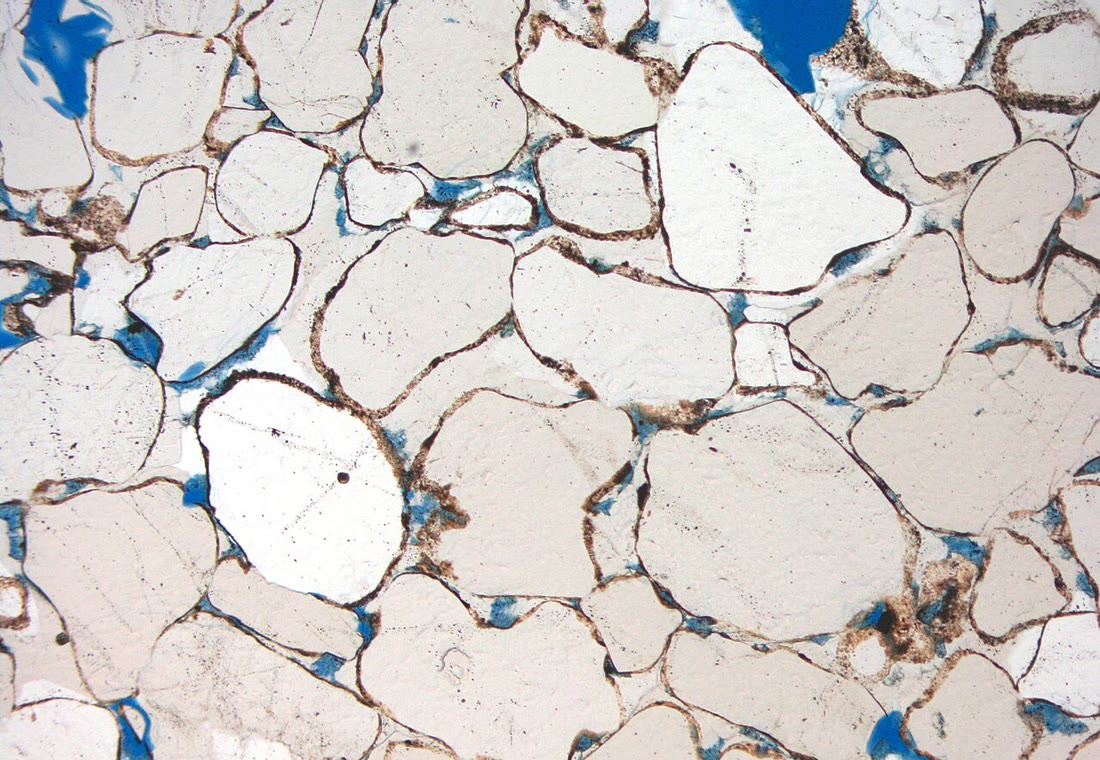
\includegraphics[width=0.62\linewidth]{images/book3/b1-quartz-overgrowths.jpg}

{\small न्यूयॉर्क राज्य के पॉट्सडैम बलुआ पत्थर (कैम्ब्रियन) का एक पतला काट, \omterm{def:b1:field-lab-methods-1:microscope}{समतल-ध्रुवित प्रकाश} में। गोलाकार मूल कण धूल और मृत्तिका की गहरी कोरों से घिरे हैं; कोरों के बाहर का स्वच्छ क्वार्ट्ज वह \omterm{def:b1:diagenesis-basins:cement}{सीमेंट} है जो कणों पर उगा, उनके साथ प्रकाशीय निरंतरता में, जब तक पड़ोसी अतिवृद्धियाँ सीधे फलकों पर मिल न गईं। छिद्रों में जो भाग बचा है वह नीले रेज़िन से भरा है। (फ़ोटो: M.~C.~Rygel, CC~BY-SA~4.0, विकिमीडिया कॉमन्स के माध्यम से; मूल का पैमाना-पट्टी काटी गई।)}
\label{fig:b1:diagenesis-basins:overgrowths}
\end{omfigure}
% ledger: commons:potsdam

हर परिवर्तन छिद्रता नष्ट नहीं करता। वह पानी जो किसी \omterm{def:b1:rock-forming-minerals:mineral}{खनिज} से असंतृप्त है, उसे घोलता है: फ़ेल्डस्पार और कार्बोनेट के कण, और पूर्व के कार्बोनेट \omterm{def:b1:diagenesis-basins:cement}{सीमेंट} हटाए जा सकते हैं और एक द्वितीयक छिद्रता छोड़ते हैं, ऐसे छिद्र जो उन कणों के आकार के हों जिन्हें वे प्रतिस्थापित करते हैं। \omterm{def:b1:weathering-clays:clay-mineral}{मृत्तिका-खनिज} बदले में छिद्रों में उगते हैं, कणों पर परतों के रूप में, या ऐसे क्रिस्टलों के रूप में जो छिद्रों को भरते हैं और उनके बीच के मार्गों को सँकरा करते हैं, जिससे पारगम्यता घटती है। तलछट के \omterm{def:b1:rock-forming-minerals:mineral}{खनिज} भी बदलते हैं: सीपियों और \omterm{def:b1:chemical-biogenic-sediments:factory}{कार्बोनेट कारखाने} का ऐरागोनाइट कैल्साइट में लौट जाता है, जो सतह पर स्थिर है, और मैग्नीशियम युक्त पानी की उपस्थिति में कैल्साइट डोलोमाइट बन सकता है।
% ledger: og:diagenesis

कैल्साइट का डोलोमाइट से प्रतिस्थापन, डोलोमिटीकरण, पानी के मैग्नीशियम के साथ एक अभिक्रिया है,
\[
  \ce{2 CaCO3 + Mg^2+ -> CaMg(CO3)2 + Ca^2+},
\]
और यह ठोस के आयतन को बदल देती है।

\begin{proposition}[डोलोमिटीकरण छिद्रता बनाता है]\label{prop:b1:diagenesis-basins:dolomite}
यदि घनत्व $\rho_c$ के दो मोल कैल्साइट को घनत्व $\rho_d$ के एक मोल डोलोमाइट से प्रतिस्थापित किया जाए, तो ठोस का आयतन इस अंश से घटता है
\[
  1 - \frac{M_d/\rho_d}{2M_c/\rho_c},
\]
जहाँ $M_c$ और $M_d$ मोलर द्रव्यमान हैं। $\rho_c = \qty{2.71}{g.cm^{-3}}$ और
$\rho_d = \qty{2.84}{g.cm^{-3}}$ के साथ यह अंश \qty{12.1}{\percent} है।
\end{proposition}

\begin{proof}
किसी \omterm{def:b1:rock-forming-minerals:mineral}{खनिज} का मोलर आयतन उसके मोलर द्रव्यमान को उसके घनत्व से भाग देने पर मिलता है। दो मोल कैल्साइट $2M_c/\rho_c$ घेरते हैं और एक मोल डोलोमाइट, वह $M_d/\rho_d$; खोया हुआ अंश उनके अनुपात का एक से अंतर है।
$M_c = \qty{100.09}{g.mol^{-1}}$ और $M_d = \qty{184.40}{g.mol^{-1}}$ के साथ दो आयतन ये हैं
$2\times\qty{36.93}{cm^3} = \qty{73.86}{cm^3}$ और \qty{64.93}{cm^3}, और
$1 - 64.93/73.86 = \num{0.121}$।
\end{proof}

यदि शैल का बाहरी आयतन नहीं बदलता, तो ठोस की हानि छिद्र-स्थान का लाभ है: \num{0.10} छिद्रता वाला एक चूना-पत्थर, जो मोल-दर-मोल डोलोमाइट से प्रतिस्थापित हो, लगभग \num{0.21} छिद्रता पाता है। अभिक्रिया के लिए बहुत अधिक मैग्नीशियम चाहिए, जिसे समुद्री जल लगभग \qty{1.28}{g} प्रति किलोग्राम रखता है; वह उन स्थानों पर तरजीह पाती है जहाँ ब्राइन या समुद्री जल चट्टान से लंबे समय तक बहते हैं (\cref{exo:b1:diagenesis-basins:12})।
% ledger: hom:calcite, webmineral:others, teos10:reference-composition, teos10:reference-salinity

\omterm{def:b1:diagenesis-basins:diagenesis}{डायाजेनेसिस} तलछट के इतिहास का अनुसरण करता है। निक्षेपण के ठीक बाद, सतह के पास, छिद्र-जल अब भी समुद्र, झील या वर्षा का है: तलछट में बिल बने होते हैं, वे समुद्र-तल पर या मिट्टी में जल्दी सीमेंटित होते हैं, और ऐरागोनाइट कैल्साइट में बदलता है। दफ़न और ऊष्मन के साथ \omterm{def:b1:diagenesis-basins:compaction}{संपीड़न}, दाब-विलयन और क्वार्ट्ज \omterm{def:b1:diagenesis-basins:cement}{सीमेंट} प्रमुख हो जाते हैं। यदि द्रोणी बाद में ऊपर उठकर अपरदित हो जाए, तो सतह से ताज़ा पानी चट्टानों में वापस बहता है और फिर से कार्बोनेट और फ़ेल्डस्पार घोलता है। एक पतला काट इन घटनाओं का क्रम दर्ज करता है: घुले कण द्वारा छोड़े गए छिद्र को भरने वाला \omterm{def:b1:diagenesis-basins:cement}{सीमेंट} घुलने से छोटा है, और संपीड़न से टूटी अतिवृद्धि उससे पुरानी है।

\section{अवसादी द्रोणियाँ}\label{sec:b1:diagenesis-basins:basins}

किलोमीटर मोटा तलछट केवल वहीं जमा होता है जहाँ फ़र्श लगातार धँसता रहता है।

\begin{definition}[अवसादी द्रोणी]\label{def:b1:diagenesis-basins:basin}
एक \emph{अवसादी द्रोणी}\index{अवसादी द्रोणी} पृथ्वी की सतह का एक क्षेत्र है जहाँ पपड़ी लंबे समय तक, कुछ मिलियन से कुछ सौ मिलियन वर्षों तक, धँसी है, और जहाँ इस प्रकार बनी जगह तलछट से भरी गई है, जो सैकड़ों मीटर से लेकर कई किलोमीटर मोटी है।
\end{definition}

\begin{definition}[अवधसान, विवर्तनिक अवधसान]\label{def:b1:diagenesis-basins:subsidence}
किसी द्रोणी का \emph{अवधसान}\index{अवधसान} उसके आधार-तल का, उस सतह का जिस पर उसके तलछट टिकते हैं, नीचे की ओर गति है, जो पृथ्वी के केंद्र जैसे एक स्थिर संदर्भ से मापी जाती है। उसका \emph{विवर्तनिक अवधसान}\index{विवर्तनिक अवधसान} वह भाग है जो उन प्रक्रियाओं से आता है जो द्रोणी बनाती हैं, उस अतिरिक्त धँसाव से भिन्न जो उसे भरने वाले तलछट और पानी के भार से होता है; इसे उस अवधसान से मापा जाता है जो आधार-तल केवल पानी के भार के अंतर्गत पाता।
\end{definition}

फ़र्श को क्या धँसाता है, वह प्लेट में द्रोणी का स्थान है (नीचे का चित्र)।

\begin{description}
  \item[दरार-द्रोणियाँ।] \omterm{def:b1:faults-folds-fabrics:fault-types}{सामान्य भ्रंश} पपड़ी को खींचते हैं, और उनके बीच के खंड नीचे धँसते हैं (\cref{ch:b1:rifts-ridges-margins})। द्रोणियाँ सँकरी और असममित हैं, और \omterm{def:b1:rifts-ridges-margins:rift}{अर्ध-ग्राबेन} अपने सीमा-भ्रंश के सामने सबसे तेज़ी से भरते हैं। उत्तरी सागर के तेल-क्षेत्र उसके वाइकिंग और केंद्रीय \omterm{def:b1:rifts-ridges-margins:rift}{ग्राबेन} की संरचनाओं में हैं, जो युवा तलछटों के नीचे दबे हैं। जब खिंचाव रुकता है, तो पतला और गरम हुआ \omterm{def:b1:layered-earth:lithosphere}{स्थलमंडल} ठंडा होता है, सिकुड़ता है, और दसियों लाख वर्षों में धीरे-धीरे धँसता रहता है। उत्तरी सागर का केंद्र, जिसका आखिरी बड़ा खिंचाव मध्य-क्रिटेशियस में समाप्त हुआ, तब एक चौड़ी, तश्तरी-आकार की द्रोणी के रूप में धँसा, जिसे क्रमशः चॉक, बलुआ पत्थरों और, तृतीयक के अधिकांश भाग में, शेल और मडस्टोन ने भरा; उसका आधार-तल, केवल पानी के भार से, बीच में \qtyrange{1100}{1400}{m} धँस गया होता।
  \item[निष्क्रिय किनारे।] जहाँ दरार महासागर बन गई, वही शीतलन हर किनारे को विदारण के बाद धँसाता है, और महासागर की ओर मोटी होती तलछट की एक पच्चर पुरानी दरार-द्रोणियों के ऊपर फैलती है।
  \item[अग्रभूमि द्रोणियाँ।] किसी अधिक्षेप-पट्टी के सामने, एक-पर-एक रखी अधिक्षेप-चादरों का भार समस्थितिक रूप से \omterm{def:b1:layered-earth:lithosphere}{स्थलमंडल} को नीचे मोड़ता है, एक ऐसी द्रोणी में जो पट्टी के सबसे निकट सबसे गहरी है और उससे अपरदित मलबे से भरी है। पश्चिमी कनाडा के अधिकांश क्रिटेशियस शैल ऐसी ही एक द्रोणी में जमा हुए थे, रॉकी पर्वतों के सामने।
  \item[अंतःक्रेटॉनिक द्रोणियाँ।] पुराने महाद्वीपों के भीतरी भागों में, किसी प्लेट-सीमा से दूर, चौड़े गोल या अंडाकार क्षेत्र बहुत लंबे समय तक धीरे-धीरे धँसे हैं। पेरिस द्रोणी ऐसे ही एक संरचनात्मक अवनमन का केंद्र है, जो ब्रिटनी, मैसिफ़ सांट्रल और वोज़ और आर्देन के पुराने मैसिफ़ों के बीच स्थित है।
  \item[स्ट्राइक-स्लिप द्रोणियाँ।] जहाँ एक \omterm{def:b1:faults-folds-fabrics:fault-types}{स्ट्राइक-स्लिप भ्रंश} उस दिशा में एक ओर हटता है जो उसकी दीवारों को अलग खींचती है --- एक मुक्त करने वाला मोड़ --- पपड़ी का एक समांतर-चतुर्भुज दो भ्रंश-पट्टियों के बीच धँसता है: एक पुल-अपार्ट द्रोणी, जैसी लॉस एंजिल्स क्षेत्र की सैन-एंड्रियास प्रणाली के साथ की द्रोणियाँ हैं।
\end{description}
% ledger: ws:basins, sc80:north-sea, britannica:paris-basin

\omterm{def:b1:layered-earth:lithosphere}{स्थलमंडल} हर सेटिंग में क्यों धँसता है, किस दर से, और द्रोणियाँ एक-दूसरे से कैसे तुलना करती हैं, यह पुस्तक 4 (स्नातक वर्ष 2) का विषय है; यहाँ उन्हें इस आधार पर अलग किया जाता है कि वे कहाँ स्थित हैं और उनके भराव का आकार कैसा है।

\begin{omfigure}
\begin{tikzpicture}[font=\scriptsize, line join=round]
% (a) rift: a half-graben
\begin{scope}
  \fill[lith granite] (0,0) -- (0,1.6) -- (1.4,1.6) -- (2.2,0.2) -- (5.0,1.0) -- (5.0,0) -- cycle;
  \fill[lith shale] (1.4,1.6) -- (2.2,0.2) -- (5.0,1.0) -- (5.0,1.6) -- cycle;
  \fill[lith sandstone] (1.4,1.6) -- (1.75,0.99) -- (5.0,1.25) -- (5.0,1.6) -- cycle;
  \draw[normal fault, thick] (1.4,1.6) -- (2.3,0.0);
  \draw[black!70] (0,1.6) -- (5.0,1.6);
  \node[anchor=south west] at (0,1.65) {(a) दरार: अर्ध-ग्राबेन};
  \node[fill=white, fill opacity=0.8, text opacity=1, inner sep=1pt] at (3.9,0.3) {आधार-तल};
  \node[fill=white, fill opacity=0.8, text opacity=1, inner sep=1pt] at (0.65,0.8) {पादभित्ति};
\end{scope}
% (b) passive margin: a seaward-thickening wedge over thinned crust
\begin{scope}[xshift=6.6cm]
  \fill[lith sea] (2.0,1.6) -- (5.0,1.6) -- (5.0,0.75) -- (3.6,0.95) -- cycle;
  \fill[lith granite] (0,0) -- (0,1.2) -- (2.0,1.0) -- (3.6,0.35) -- (5.0,0.05) -- (5.0,0) -- cycle;
  \fill[lith shale] (0,1.2) -- (2.0,1.0) -- (3.6,0.35) -- (5.0,0.05) -- (5.0,0.75) -- (3.6,0.95) -- (2.0,1.6) -- (0,1.6) -- cycle;
  \draw[black!70] (0,1.6) -- (2.0,1.6) -- (3.6,0.95) -- (5.0,0.75);
  \draw[blue!60!black, thick] (2.0,1.6) -- (5.0,1.6);
  \node[anchor=south west] at (0,1.65) {(b) निष्क्रिय किनारा};
  \node[fill=white, fill opacity=0.8, text opacity=1, inner sep=1pt] at (1.0,0.45) {पतली महाद्वीपीय पपड़ी};
  \node[anchor=north east] at (5.0,1.58) {महासागर};
\end{scope}
% (c) foreland basin: asymmetric, deepest against the thrust belt
\begin{scope}[yshift=-3.3cm]
  \fill[lith granite] (0,0) -- (0,0.55) -- (5.0,1.35) -- (5.0,0) -- cycle;
  \fill[lith sandstone] (0,0.55) -- (5.0,1.35) -- (5.0,1.6) -- (0,1.6) -- cycle;
  \fill[lith conglomerate] (1.0,1.6) -- (3.6,1.6) -- (1.0,1.0) -- cycle;
  \fill[omLithSchist, draw=black!70] (0,0.95) -- (1.9,1.6) -- (1.3,1.95) -- (0.4,2.25) -- (0,2.3) -- cycle;
  \draw[thrust fault] (0,0.95) -- (1.9,1.6);
  \draw[thrust fault] (0,1.55) -- (1.15,1.95);
  \draw[black!70] (1.9,1.6) -- (5.0,1.6);
  \node[anchor=south west] at (2.0,1.65) {(c) अग्रभूमि द्रोणी};
  \node[anchor=south west, inner sep=1pt] at (0.25,2.3) {अधिक्षेप-पट्टी};
  \node[fill=white, fill opacity=0.8, text opacity=1, inner sep=1pt] at (3.9,0.35) {आधार-तल};
\end{scope}
% (d) intracratonic basin: a broad sag, layers thickening to the centre
\begin{scope}[xshift=6.6cm, yshift=-3.3cm]
  \fill[lith granite] (0,0) -- (0,1.5) .. controls (1.6,1.1) and (2.0,0.3) .. (2.5,0.3) .. controls (3.0,0.3) and (3.4,1.1) .. (5.0,1.5) -- (5.0,0) -- cycle;
  \fill[lith limestone] (0,1.5) .. controls (1.6,1.1) and (2.0,0.3) .. (2.5,0.3) .. controls (3.0,0.3) and (3.4,1.1) .. (5.0,1.5) -- (5.0,1.6) -- (0,1.6) -- cycle;
  \fill[lith shale] (0.6,1.6) .. controls (1.6,1.35) and (2.1,0.85) .. (2.5,0.85) .. controls (2.9,0.85) and (3.4,1.35) .. (4.4,1.6) -- cycle;
  \fill[lith sandstone] (1.3,1.6) .. controls (1.9,1.5) and (2.2,1.3) .. (2.5,1.3) .. controls (2.8,1.3) and (3.1,1.5) .. (3.7,1.6) -- cycle;
  \draw[black!70] (0,1.6) -- (5.0,1.6);
  \node[anchor=south west] at (0,1.65) {(d) अंतःक्रेटॉनिक द्रोणी};
  \node[fill=white, fill opacity=0.8, text opacity=1, inner sep=1pt] at (4.2,0.4) {आधार-तल};
\end{scope}
\end{tikzpicture}

{\small चार प्रकार की अवसादी द्रोणियाँ अनुप्रस्थ काट में (योजनाबद्ध, पैमाने पर नहीं; ऊर्ध्वाधर पैमाना बढ़ाकर)। (a)~एक दरार: \omterm{def:b1:rifts-ridges-margins:rift}{अर्ध-ग्राबेन} की सीमा-भ्रंश के सामने भराव मोटा होता है। (b)~एक \omterm{def:b1:rifts-ridges-margins:passive-margin}{निष्क्रिय किनारा}: पतली महाद्वीपीय पपड़ी के ऊपर तलछट की एक पच्चर, जो महासागर की ओर मोटी होती है। (c)~एक अग्रभूमि द्रोणी, जो अधिक्षेप-पट्टी के सबसे निकट सबसे गहरी है, जिसका भार उसे नीचे मोड़ता है, और जो उसके मलबे से भरी है, सबसे मोटा (कंग्लोमरेट) पट्टी के निकट; पट्टी अपनी ही द्रोणी के किनारे पर चढ़ जाती है। (d)~एक अंतःक्रेटॉनिक द्रोणी: एक चौड़ा अवनमन जिसकी परतें केंद्र की ओर मोटी होती हैं।}
\label{fig:b1:diagenesis-basins:types}
\end{omfigure}

\begin{inthefield}[द्रोणियाँ कैसे जानी जाती हैं]
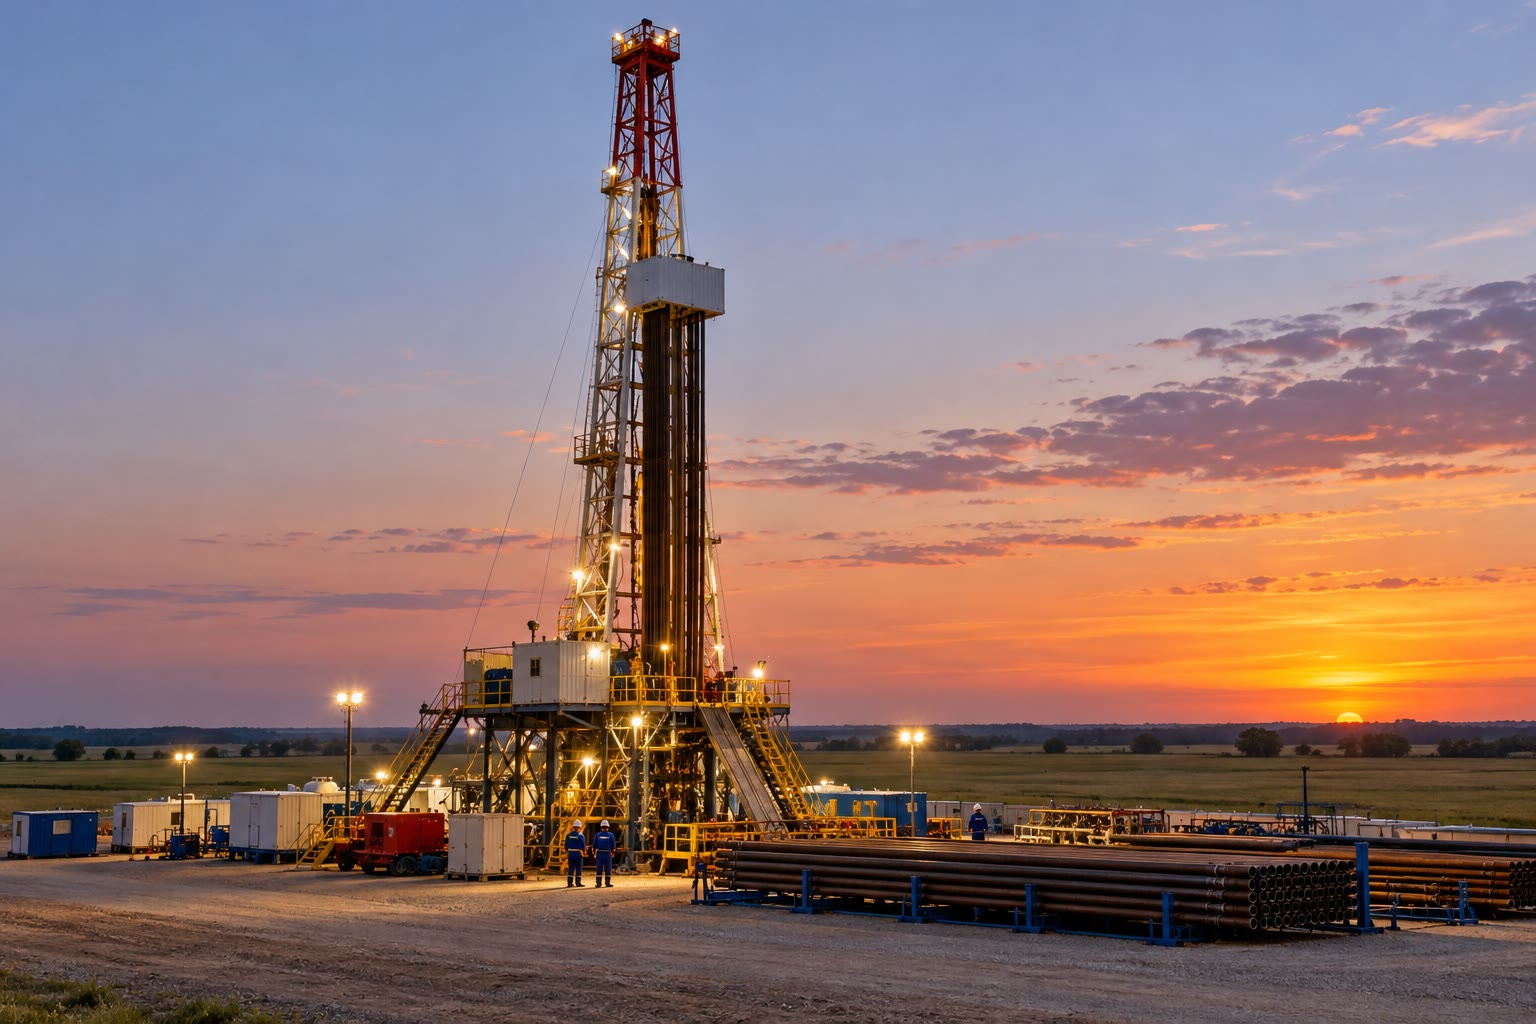
\includegraphics[width=0.3\linewidth]{images/book3/ai/b1-drilling-rig.jpg}\hfill
\begin{minipage}[b]{0.67\linewidth}
लगभग हर वह बात जो किसी द्रोणी के गहरे भराव के बारे में ज्ञात है, तेल, गैस और पानी की खोज से आती है। भूकंपीय परावर्तन सर्वेक्षण हज़ारों वर्ग किलोमीटर पर उसकी परतों और भ्रंशों का चित्र लेते हैं; कुएँ उसका नमूना एक बिंदु पर लेते हैं। एक कुआँ बिट द्वारा काटे गए शैल के टुकड़े लौटाता है, अंतरालों पर कोर, और छेद के चारों ओर की चट्टानों के भौतिक गुणों के सतत लॉग, जिनसे छिद्रता हर मीटर पर पढ़ी जाती है। एथी के नियम के छिद्रता-गहराई वक्र, और द्रोणियों के \omterm{def:b1:diagenesis-basins:subsidence}{अवधसान} इतिहास, पहली बार ऐसे ही कुओं से बने।
\end{minipage}

\smallskip
{\small संध्या समय एक भूमि ड्रिलिंग रिग, अग्रभूमि में रैकों पर चढ़ाए गए पाइप सहित (AI से बनाया गया चित्र)।}
\end{inthefield}
% ledger: sc80:north-sea

\section{अवधसान, आवास-स्थान और समुद्र-स्तर}\label{sec:b1:diagenesis-basins:accommodation}

तलछट केवल वहीं ढेर लग सकता है जहाँ उसके लिए ऐसी जगह हो जो उस स्तर से नीचे हो जिस पर वह आगे हटाया जाता। समुद्र में वह स्तर समुद्र-स्तर के लगभग पास है, और जगह दो गतियों का मामला है: फ़र्श की, और समुद्र की सतह की।

\begin{definition}[आवास-स्थान]\label{def:b1:diagenesis-basins:accommodation}
किसी द्रोणी के एक बिंदु पर \emph{आवास-स्थान}\index{आवास-स्थान} वह स्थान है जो वहाँ तलछट के जमा होने के लिए उपलब्ध है: तलछट की ऊपरी सतह से समुद्र-स्तर तक की ऊर्ध्वाधर दूरी, समुद्री निक्षेपण का आधार-स्तर। एक समय-अंतराल में बना आवास-स्थान आधार-तल से जुड़े एक संदर्भ-बिंदु से समुद्र-स्तर तक की दूरी में वृद्धि है।
\end{definition}

\begin{definition}[यूस्टेसी, सापेक्ष समुद्र-स्तर]\label{def:b1:diagenesis-basins:eustasy}
\emph{यूस्टेसी}\index{यूस्टेसी} विश्व महासागर के स्तर का परिवर्तन है, जो एक स्थिर संदर्भ, पृथ्वी के केंद्र, के सापेक्ष मापा जाता है, और महासागर में या महासागर-द्रोणियों के आयतन में पानी के आयतन के परिवर्तन से होता है; वह हर जगह एक-सा है। किसी स्थान पर \emph{सापेक्ष समुद्र-स्तर}\index{सापेक्ष समुद्र-स्तर} वहाँ आधार-तल से जुड़े एक आंकड़े के ऊपर समुद्र की सतह की ऊँचाई है; वह यूस्टेसी से और भूमि की ऊर्ध्वाधर गति से बदलती है।
\end{definition}

\begin{proposition}[आवास-स्थान का बजट]\label{prop:b1:diagenesis-basins:budget}
एक समय-अंतराल में मान लीजिए $\Delta E$ समुद्र-स्तर की \omterm{def:b1:diagenesis-basins:eustasy}{यूस्टेसी} वृद्धि है और $S$ आधार-तल का \omterm{def:b1:diagenesis-basins:subsidence}{अवधसान} (समुद्र के लिए दोनों ऊपर की ओर धनात्मक, फ़र्श के लिए नीचे की ओर)। बना \omterm{def:b1:diagenesis-basins:accommodation}{आवास-स्थान} है
\[
  \Delta A = \Delta E + S ,
\]
और वह जोड़ी गई तलछट की मोटाई के बीच बँटता है, जो संदर्भ के ऊपर $\Delta T$ है, और पानी की गहराई में वृद्धि, $\Delta W$: $\Delta E + S = \Delta T + \Delta W$।
\end{proposition}

\begin{proof}
आंकड़े निश्चित संदर्भ से मापिए। मान लीजिए $e$ समुद्र की सतह की ऊँचाई है, $b$ आंकड़े की, $T$ आंकड़े के ऊपर तलछट की मोटाई, और $W$ तलछट के ऊपर पानी की गहराई, ताकि $e = b + T + W$ हो।
\omterm{def:b1:diagenesis-basins:eustasy}{सापेक्ष समुद्र-स्तर} $R = e - b = T + W$ है। इस अंतराल में $\Delta e =
\Delta E$ और $\Delta b = -S$ है, इसलिए $\Delta R = \Delta E + S$; और $\Delta R =
\Delta T + \Delta W$।
\end{proof}

समुद्र-तल जो निश्चित गहराई पर रखा गया हो ($\Delta W = 0$), उतनी ही तेज़ी से भरता है जितनी तेज़ी से \omterm{def:b1:diagenesis-basins:accommodation}{आवास-स्थान} बनता है; जो उथला होता है वह तेज़ी से भरता है, और तट समुद्र की ओर खिसकता है; जो गहरा होता है वह भूखा रहता है। $\Delta T$ पूरे ढेर की, संदर्भ के ऊपर, मोटाई का परिवर्तन है: यह नई जमी तलछट को गिनता है, घटाकर नीचे की पुरानी तलछटों का पतला होना जैसे-जैसे वे संपीड़ित होती हैं, इसलिए \omterm{def:b1:diagenesis-basins:compaction}{संपीड़न} स्वयं तलछट के लिए जगह बनाता है (नीचे का चित्र)।

\begin{omfigure}
\begin{tikzpicture}[font=\footnotesize, >=Stealth]
\def\col#1#2#3#4#5{% x, datum, sediment top, sea, label
  \fill[lith granite] (#1,0.2) rectangle ++(1.4,#2-0.2);
  \fill[lith shale] (#1,#2) rectangle ++(1.4,#3-#2);
  \fill[lith sea] (#1,#3) rectangle ++(1.4,#4-#3);
  \draw[black!70] (#1,#2) -- ++(1.4,0);
  \draw[blue!60!black, thick] (#1-0.2,#4) -- ++(1.8,0);
  \node[anchor=north] at (#1+0.7,0.15) {#5};}
\draw[black!60, dash dot] (-0.6,0.9) -- (8.6,0.9) node[anchor=west, align=left] {स्थिर\\ संदर्भ};
\col{0}{1.5}{3.0}{3.6}{समय $t_1$}
\col{4.4}{1.0}{3.4}{3.9}{समय $t_2$}
% eustasy
\draw[<->, omThm] (3.0,0.9) -- (3.0,3.6) node[midway, fill=white, inner sep=1pt] {$e_1$};
\draw[<->, omThm] (7.4,0.9) -- (7.4,3.9) node[midway, fill=white, inner sep=1pt] {$e_2$};
% subsidence of the datum
\draw[dashed, black!60] (1.4,1.5) -- (4.4,1.5);
\draw[->, thick] (4.2,1.5) -- (4.2,1.0) node[midway, anchor=east] {$S$};
% relative sea level
\draw[<->] (-0.35,1.5) -- (-0.35,3.6) node[midway, anchor=east] {$R_1$};
\draw[<->] (6.05,1.0) -- (6.05,3.9) node[midway, anchor=west] {$R_2$};
\node[anchor=west] at (1.5,2.25) {$T_1$};
\node[anchor=west] at (1.5,3.3) {$W_1$};
\node at (5.1,2.2) {$T_2$};
\node at (5.1,3.65) {$W_2$};
\node[anchor=south, align=center, blue!60!black] at (5.1,3.95) {समुद्र-स्तर};
\node[anchor=west, align=left, font=\scriptsize] at (8.6,2.4) {$R = e - b = T + W$\\[2pt] $\Delta R = \Delta E + S$\\ $\phantom{\Delta R} = \Delta T + \Delta W$};
\end{tikzpicture}

{\small दो समयों पर एक ही स्थान पर \omterm{def:b1:diagenesis-basins:accommodation}{आवास-स्थान} (योजनाबद्ध)। $t_1$ और $t_2$ के बीच समुद्र-स्तर स्थिर संदर्भ से ऊपर $\Delta E = e_2 - e_1$ बढ़ता है और आधार-तल $S$ धँसता है: \omterm{def:b1:diagenesis-basins:eustasy}{सापेक्ष समुद्र-स्तर} $R$ बना \omterm{def:b1:diagenesis-basins:accommodation}{आवास-स्थान}, $\Delta E + S$, बढ़ता है, जो और तलछट ($T_2 > T_1$) और पानी की गहराई में बदलाव (यहाँ हल्का उथलापन, $W_2 < W_1$) के बीच बँटता है।}
\label{fig:b1:diagenesis-basins:accommodation}
\end{omfigure}

एक द्रोणी केवल अपने \omterm{def:b1:diagenesis-basins:subsidence}{विवर्तनिक अवधसान} से नहीं धँसती: उसे भरने वाली तलछट एक भार है, और \omterm{def:b1:layered-earth:lithosphere}{स्थलमंडल} उसके नीचे और धँसता है।

\begin{proposition}[तलछट का भार अवधसान बढ़ाता है]\label{prop:b1:diagenesis-basins:loading}
स्थानीय (एरी) समस्थितिक संतुलन में, घनत्व $\rho_m$ के मैंटल पर, एक द्रोणी जिसका आधार-तल, केवल घनत्व $\rho_w$ के पानी के भार से, समुद्र-स्तर के नीचे गहराई $Y$ पर होता, समुद्र-स्तर तक औसत घनत्व $\rho_s$ वाले तलछट से भरे जाने पर, मोटाई
\[
  h = Y\,\frac{\rho_m - \rho_w}{\rho_m - \rho_s}
\]
का तलछट रखती है। भूमि पर, जहाँ ऊपर वायु है और भराव परिवेश के स्तर तक है, गुणक $\rho_m/(\rho_m - \rho_s)$ है।
\end{proposition}

\begin{proof}
एक ही \omterm{def:b1:layered-earth:lithosphere}{स्थलमंडल} वाले दो स्तंभों की तुलना कीजिए, प्रति इकाई क्षेत्रफल द्रव्यमान $M$ और मोटाई $L$, दोनों के नीचे एक संतुलन-गहराई $z_c$ तक। पानी से भरा स्तंभ $\rho_w Y + M + \rho_m(z_c - Y - L)$ रखता है; तलछट से भरा $\rho_s h + M + \rho_m(z_c - h - L)$। \cref{prop:b1:isostasy-gravity:equal-mass} से दोनों द्रव्यमान बराबर हैं, इसलिए
$\rho_w Y - \rho_m Y = \rho_s h - \rho_m h$, अर्थात् $h(\rho_m - \rho_s) =
Y(\rho_m - \rho_w)$। पानी के स्थान पर वायु हो तो $\rho_w$ को शून्य से बदल दिया जाता है।
\end{proof}

$\rho_m = \qty{3300}{kg.m^{-3}}$, $\rho_w = \qty{1030}{kg.m^{-3}}$ और औसत घनत्व \qty{2300}{kg.m^{-3}} वाला तलछट लेकर, इनसे गुणक $2270/1000 = \num{2.27}$ है: एक द्रोणी जिसका \omterm{def:b1:diagenesis-basins:subsidence}{विवर्तनिक अवधसान} \qty{1}{km} पानी के लिए जगह बनाता, \qty{2.27}{km} तलछट रखती है। भूमि पर गुणक $3300/1000 = \num{3.3}$ होता। भराव का घनत्व स्थिर नहीं है: वह तलछट के संपीड़ित होने के साथ बढ़ता है, और गुणक भी, इसलिए तलछट की मोटाई को \omterm{def:b1:diagenesis-basins:subsidence}{विवर्तनिक अवधसान} में बदलने के लिए हर परत का \omterm{def:b1:diagenesis-basins:compaction}{डिकंपैक्शन} चाहिए, समय-चरण दर समय-चरण। वह प्रक्रिया, बैकस्ट्रिपिंग, पुस्तक 4 (स्नातक वर्ष 2) में आती है।

समुद्र-स्तर स्वयं भी स्थिर नहीं है। अंतिम हिमनद उच्चिष्ठ पर बर्फ़ की चादरों ने उत्तरी अमेरिका और उत्तरी यूरोप का बड़ा भाग ढका था, और उनमें बंद पानी महासागर से लिया गया था। ठोस पृथ्वी की बदलते बर्फ़ और पानी के भारों पर प्रतिक्रिया के लिए सुधार करने पर, पूर्व तटरेखाओं के प्रेक्षण ऐसा समुद्र-स्तर देते हैं जो लगभग \num{30000} वर्ष पहले लगभग \qty{40}{m} तेज़ी से गिरा, और फिर धीरे-धीरे, \qtyrange{29}{21}{\ka} के बीच, आज के स्तर से \qty{134}{m} नीचे तक; ज़मीन पर टिकी बर्फ़ तब आज से लगभग \qty{52e6}{km^3} अधिक थी। अक्सर उद्धृत \qty{125}{m} का आंकड़ा छोटा है, क्योंकि वह आम तौर पर इन समस्थितिक प्रभावों के लिए सुधारा नहीं जाता। हिमनद-मुक्ति मुख्यतः \qty{16.5}{\ka} और \qty{8.2}{\ka} के बीच आई, औसतन \qty{12}{m} प्रति हज़ार वर्ष, और \qty{14.5}{\ka} और \qty{14.0}{\ka} के बीच \qty{40}{mm} प्रति वर्ष या अधिक दर से।
% ledger: lambeck:lgm, lambeck:deglaciation

पुराने निम्न-स्तर गहरे-समुद्र के कोरों के फ़ोरामिनिफ़ेरा के ऑक्सीजन समस्थानिकों से पढ़े जाते हैं, जो भूमि पर बर्फ़ का आयतन दर्ज करते हैं। पिछले \num{430000} वर्षों के सात ऐसे पुनर्निर्माणों का, और पिछले \num{800000} के पाँच पुनर्निर्माणों का, औसत लेने से हर एक की त्रुटियाँ मिट जाती हैं; होलोसीन और अंतिम हिमनद निम्न-स्तर तक मापने पर स्टैक की अनिश्चितता \qtyrange{9}{12}{m} है (नीचे का चित्र)। वह हिमनद चक्रों को आरी-दाँत के रूप में दिखाता है: समुद्र-स्तर की धीमी गिरावटें, हर एक एक तेज़ उत्थान से समाप्त --- पिछले \num{800000} वर्षों में पाँच बार, \num{20000} वर्ष से कम में \qty{100}{m} से अधिक का उत्थान। इस पैमाने पर \omterm{def:b1:diagenesis-basins:eustasy}{यूस्टेसी} तट-रेखा को महाद्वीपीय शेल्फ़ों के पार आगे-पीछे खिसकाती है।
% ledger: spratt:stack, data:b3-sealevel-stack

\begin{omfigure}
\begin{tikzpicture}[font=\footnotesize]
\begin{axis}[width=16cm, height=4.8cm, xmin=0, xmax=800, ymin=-150, ymax=40,
    x dir=reverse, xlabel={आयु (हज़ार वर्ष, वर्तमान से पूर्व)}, xlabel style={yshift=2pt},
    ylabel={समुद्र-स्तर (m)}, ytick={-150,-100,-50,0},
    title={(a) पिछले \num{800000} वर्ष (पाँच अभिलेख)}, title style={font=\footnotesize},
    axis on top]
  \addplot[draw=none, name path=hi] table[x=age, y=hi] {figdata/out/bachelor-1-sea_level-long.dat};
  \addplot[draw=none, name path=lo] table[x=age, y=lo] {figdata/out/bachelor-1-sea_level-long.dat};
  \addplot[omThm!25] fill between[of=hi and lo];
  \addplot[thin, omThm] table[x=age, y=sl] {figdata/out/bachelor-1-sea_level-long.dat};
  \draw[black!50, densely dotted] (axis cs:0,0) -- (axis cs:800,0);
\end{axis}
\end{tikzpicture}

\medskip
\begin{tikzpicture}[font=\footnotesize]
\begin{axis}[width=16cm, height=4.8cm,
    xmin=0, xmax=140, ymin=-160, ymax=40, x dir=reverse,
    xlabel={आयु (हज़ार वर्ष, वर्तमान से पूर्व)}, ylabel={समुद्र-स्तर (m)},
    ytick={-150,-100,-50,0},
    title={(b) पिछले \num{140000} वर्ष (सात अभिलेख)}, title style={font=\footnotesize},
    axis on top]
  \addplot[draw=none, name path=hi] table[x=age, y=hi] {figdata/out/bachelor-1-sea_level-short.dat};
  \addplot[draw=none, name path=lo] table[x=age, y=lo] {figdata/out/bachelor-1-sea_level-short.dat};
  \addplot[omThm!25] fill between[of=hi and lo];
  \addplot[thick, omThm] table[x=age, y=sl] {figdata/out/bachelor-1-sea_level-short.dat};
  \draw[black!50, densely dotted] (axis cs:0,0) -- (axis cs:140,0);
  \addplot[only marks, mark=*, mark size=1.6pt, black] coordinates {(21,-134)};
  \draw[black!60, thin] (axis cs:21,-131) -- (axis cs:21,-46);
  \node[anchor=south, font=\scriptsize, fill=white, inner sep=1pt] at (axis cs:36,-46) {\qty{-134}{m}, \qty{21}{\ka} पर, तटरेखाओं से (लैम्बेक और सहलेखक, 2014)};
\end{axis}
\end{tikzpicture}

{\small स्प्रैट और लिसीकी (2016) के स्टैक से वर्तमान के सापेक्ष वैश्विक समुद्र-स्तर: गहरे-समुद्र के कोरों से पाँच पुनर्निर्माणों का पहला मुख्य घटक, \num{800000} वर्षों पर (a), और पिछले \num{140000} वर्षों के सात का (b), उसकी एक-मानक-विचलन पट्टी के साथ। स्टैक का निम्नतम मान, \qty{24}{\ka} पर \qty{-130}{m}, पूर्व तटरेखाओं से मिले \qty{-134}{m} (बिंदु) की उस पट्टी के भीतर है; अंतिम अंतर्हिमनद \qty{121}{\ka} पर आज से लगभग \qty{3}{m} ऊँचा है। डेटा: NOAA NCEI World Data Service for Paleoclimatology।}
\label{fig:b1:diagenesis-basins:sea-level}
\end{omfigure}
% computed in figdata/bachelor-1/sea_level.py; ledger: data:b3-sealevel-stack, spratt:stack, lambeck:lgm

किसी द्रोणी के जीवनकाल में ऐसे उतार-चढ़ाव संक्षिप्त होते हैं। कुछ दसियों हज़ार वर्षों में \qty{100}{m} से अधिक का हिमनद-पतन, \omterm{def:b1:diagenesis-basins:subsidence}{विवर्तनिक अवधसान} की तुलना में तेज़ और बड़ा है, जो केवल दसियों लाख वर्षों में एक किलोमीटर या अधिक जुड़ता है; पर हिमनद उतार-चढ़ाव लगभग \qty{150}{m} की सीमा में रहते हैं, इसलिए द्रोणी के मोटे भराव में जगह का अधिकांश भाग \omterm{def:b1:diagenesis-basins:subsidence}{अवधसान} बनाता है, और \omterm{def:b1:diagenesis-basins:eustasy}{यूस्टेसी} उसकी परतों की लय तय करती है।
% ledger: data:b3-sealevel-stack, sc80:north-sea

\section{अभ्यास}

\begin{exercise}[$\star$]\label{exo:b1:diagenesis-basins:1}
\cref{tab:b1:diagenesis-basins:athy} के प्राचलों से, \qty{2000}{m} पर बलुआ पत्थर और शेल की छिद्रता परिकलित कीजिए। किस गहराई पर हर एक की छिद्रता अपने सतही मान के आधे तक गिर गई है?
% ledger: pybacktrack:compaction
\end{exercise}

\begin{exercise}[$\star$]\label{exo:b1:diagenesis-basins:2}
एक समय-अंतराल में समुद्र-स्तर \omterm{def:b1:diagenesis-basins:eustasy}{यूस्टेसी} से \qty{30}{m} बढ़ता है, एक शेल्फ़ का आधार-तल \qty{50}{m} धँसता है, और आधार-तल पर एक संदर्भ के ऊपर \qty{60}{m} तलछट जुड़ते हैं। \cref{prop:b1:diagenesis-basins:budget} से बना \omterm{def:b1:diagenesis-basins:accommodation}{आवास-स्थान} और पानी की गहराई का परिवर्तन परिकलित कीजिए। क्या शेल्फ़ गहरा होता है या उथला?
\end{exercise}

\begin{exercise}[$\star$]\label{exo:b1:diagenesis-basins:3}
द्रोणी का \omterm{def:b1:diagenesis-basins:subsidence}{विवर्तनिक अवधसान} \qty{1.0}{km} पानी के लिए जगह बनाएगा। $\rho_m = \qty{3300}{kg.m^{-3}}$ और $\rho_w = \qty{1030}{kg.m^{-3}}$ लेकर, यदि उसे समुद्र-स्तर तक भरने वाले तलछट का औसत घनत्व \qty{2300}{kg.m^{-3}} है, तो वह कितना मोटा है? \qty{2500}{kg.m^{-3}}? सघन भराव मोटी परत क्यों देता है?
\end{exercise}

\begin{exercise}[$\star$]\label{exo:b1:diagenesis-basins:4}
कैल्साइट का मोलर द्रव्यमान \qty{100.09}{g.mol^{-1}} और घनत्व \qty{2.71}{g.cm^{-3}} है; डोलोमाइट का \qty{184.40}{g.mol^{-1}} और \qty{2.84}{g.cm^{-3}}। (क)~हर एक का मोलर आयतन परिकलित कीजिए। (ख)~जब दो मोल कैल्साइट एक मोल डोलोमाइट बनते हैं, तो ठोस का आयतन किस अंश से बदलता है? (ग)~\num{0.10} छिद्रता वाला एक चूना-पत्थर मोल-दर-मोल डोलोमिटीकृत होता है, उसके बाहरी आयतन में परिवर्तन के बिना। उसकी नई छिद्रता क्या है?
% ledger: hom:calcite, webmineral:others
\end{exercise}

\begin{exercise}[$\star\star$]\label{exo:b1:diagenesis-basins:5}
एक शेल बेसिन के ऊपरी \qty{1000}{m} पर है। (क)~उसकी ठोस मोटाई और औसत छिद्रता परिकलित कीजिए। (ख)~उसे इतना दबाया जाता है कि उसका ऊपरी सिरा \qty{2000}{m} पर हो। \cref{met:b1:diagenesis-basins:decompaction} का उपयोग करके, ऊपरी सिरे को ऊपर की बजाय नीचे खिसकाकर, उसकी नई मोटाई और औसत छिद्रता ज्ञात कीजिए। (ग)~शेल का हर वर्ग मीटर कितना पानी निष्कासित कर चुका है?
% ledger: pybacktrack:compaction
\end{exercise}

\begin{exercise}[$\star\star$]\label{exo:b1:diagenesis-basins:6}
एक बलुआ पत्थर \qty{2500}{m} और \qty{2800}{m} के बीच है। (क)~उसकी ठोस मोटाई परिकलित कीजिए। (ख)~\cref{met:b1:diagenesis-basins:decompaction} से उसे सतह तक डिकंपैक्ट कीजिए, $b_0 = \qty{300}{m}$ से शुरू करते हुए हर न्यूटन चरण लिखिए। (ग)~दफ़न ने उसे कितने गुना पतला किया है?
% ledger: pybacktrack:compaction
\end{exercise}

\begin{exercise}[$\star\star$]\label{exo:b1:diagenesis-basins:7}
अंतिम हिमनद उच्चिष्ठ पर, ज़मीन पर टिकी बर्फ़ में आज से लगभग \qty{52e6}{km^3} अधिक थी। बर्फ़ का घनत्व \qty{916.7}{kg.m^{-3}}, पिघले पानी का \qty{1000}{kg.m^{-3}}, और आज के महासागर का क्षेत्रफल \qty{361.84e6}{km^2} लीजिए। (क)~यह बर्फ़ समुद्र-स्तर में कितनी गिरावट दर्शाती है? (ख)~पूर्व तटरेखाओं से पाए गए \qty{134}{m} से तुलना कीजिए। (ग)~कितना महासागर-क्षेत्र ठीक \qty{134}{m} देता, और हिमनद महासागर छोटा क्यों था?
% ledger: lambeck:lgm, iapws:ice-density, charette:ocean-volume
\end{exercise}

\begin{exercise}[$\star\star$]\label{exo:b1:diagenesis-basins:8}
समुद्र-स्तर स्टैक \qty{16}{\ka} पर \qty{-98.1}{m} और \qty{8}{\ka} पर \qty{-9.1}{m} देता है। (क)~प्रति हज़ार वर्ष मीटरों में उत्थान की औसत दर परिकलित कीजिए, और मुख्य हिमनद-मुक्ति के लिए पूर्व तटरेखाओं से पाई गई \qty{12}{m} प्रति हज़ार वर्ष से तुलना कीजिए। (ख)~\qty{14.5}{\ka} और \qty{14.0}{\ka} के बीच समुद्र-स्तर \qty{40}{mm} प्रति वर्ष या अधिक दर से उठा। औसत का कितना गुना है वह, और उन पाँच सौ वर्षों में समुद्र-स्तर कितना उठा?
% ledger: data:b3-sealevel-stack, lambeck:deglaciation
\end{exercise}

\begin{exercise}[$\star\star$]\label{exo:b1:diagenesis-basins:9}
एक शेल्फ़ \qty{20}{m} पानी के नीचे है। उसका आधार-तल \qty{50}{m} प्रति दस लाख वर्ष की दर से धँसता है। (क)~दो दस लाख वर्षों में \omterm{def:b1:diagenesis-basins:eustasy}{यूस्टेसी} से समुद्र-स्तर \qty{40}{m} गिरता है, जबकि पानी की गहराई वही रहती है। कितना \omterm{def:b1:diagenesis-basins:accommodation}{आवास-स्थान} बनता है, और कितना तलछट जुड़ता है? (ख)~फिर, किसी हिमनद के आरंभ पर, \num{20000} वर्षों में समुद्र-स्तर \qty{120}{m} गिरता है, और कोई तलछट नहीं जुड़ता। अंत में पूर्व समुद्र-तल समुद्र-स्तर से कितना ऊँचा खड़ा है?
\end{exercise}

\begin{exercise}[$\star\star\star$]\label{exo:b1:diagenesis-basins:10}
(क)~दिखाइए कि मोटाई $h$ की एक परत, गहराई $z$ पर, जो क्षय-लंबाई $\lambda$ की तुलना में पतली है, सतह पर लौटाए जाने पर मोटाई $h_0 \approx h\,(1 - \varphi(z))/(1 -
\varphi_0)$ रखती है। (ख)~इसे \qty{3000}{m} पर \qty{10}{m} शेल पर लागू कीजिए, और सटीक \omterm{def:b1:diagenesis-basins:compaction}{डिकंपैक्शन}, \qty{23.1}{m}, से तुलना कीजिए। (ग)~सन्निकटन थोड़ा अधिक बड़ा क्यों है?
% ledger: pybacktrack:compaction
\end{exercise}

\begin{exercise}[$\star\star\star$]\label{exo:b1:diagenesis-basins:11}
एक बेसिन को समुद्र-स्तर तक \qty{3000}{m} शेल से भरा गया है, जो एथी के नियम से संपीड़ित है, उसकी छिद्राएँ घनत्व \qty{1030}{kg.m^{-3}} के पानी से भरी हैं। (क)~भराव की औसत छिद्रता और औसत घनत्व परिकलित कीजिए। (ख)~\cref{prop:b1:diagenesis-basins:loading} और $\rho_m =
\qty{3300}{kg.m^{-3}}$ से भार-गुणक और वह जल-भारित \omterm{def:b1:diagenesis-basins:subsidence}{अवधसान} परिकलित कीजिए जो भराव दर्शाता है। (ग)~कणों का घनत्व, \qty{2700}{kg.m^{-3}}, लेने से गुणक बहुत बड़ा क्यों होगा, और वह गलत क्यों होगा?
% ledger: pybacktrack:compaction
\end{exercise}

\begin{exercise}[$\star\star\star$]\label{exo:b1:diagenesis-basins:12}
एक घन मीटर \num{0.10} छिद्रता वाले चूना-पत्थर को पूरी तरह, मोल-दर-मोल, डोलोमिटीकृत किया जाना है। समुद्री जल में प्रति किलोग्राम \qty{35.165}{g} लवण है, जिसमें भार-अंश \num{0.0365} मैग्नीशियम (\qty{24.305}{g.mol^{-1}}) है। (क)~घन में कितने मोल कैल्साइट हैं (\cref{exo:b1:diagenesis-basins:4} के मोलर आयतन से)? (ख)~अभिक्रिया को कितने मोल मैग्नीशियम चाहिए? (ग)~यदि घन अपना सारा मैग्नीशियम दे, तो उसके भीतर से समुद्री जल (\qty{1030}{kg.m^{-3}}) का कितना द्रव्यमान और आयतन बहना चाहिए? (घ)~उत्तर बताता है कि डोलोमाइट कहाँ बनता है?
% ledger: teos10:reference-composition, teos10:reference-salinity, hom:calcite
\end{exercise}

\section{समस्या: द्रोणी के भराव का डिकंपैक्शन}

\begin{problem}[{सप्ताहांत समस्या --- एक कुएँ के तलछट जब जमे थे तब कितने मोटे थे,
और उनके लिए जगह कैसे बनी}]
\label{pb:b1:diagenesis-basins:1}
% values: calc/ch23.py; the well, its units, ages and the eustatic changes are invented
एक कुआँ तटीय मैदान पर, समुद्र-स्तर पर खोदा गया, \qty{3200}{m} पर आधार-तल तक पहुँचने से पहले तीन इकाइयों से होकर गुज़रता है:
\begin{center}
\begin{tabular}{llll}
\hline
इकाई & शैल-प्रकार & आज की गहराई (m) & निक्षेपण का समय \\
\hline
1 & बलुआ पत्थर & 0--800     & \qtyrange{15}{0}{\Ma} \\
2 & शेल     & 800--2600  & \qtyrange{55}{15}{\Ma} \\
3 & चॉक & 2600--3200 & \qtyrange{75}{55}{\Ma} \\
\hline
\end{tabular}
\end{center}
मूल प्राचल \cref{tab:b1:diagenesis-basins:athy} से लीजिए, छिद्र-जल का घनत्व \qty{1030}{kg.m^{-3}}, $g = \qty{9.81}{m.s^{-2}}$, और मान लीजिए कि हर इकाई एथी के नियम से, उसका पानी निकलने के लिए स्वतंत्र, अपने पूरे इतिहास में संपीड़ित हुई। सूक्ष्म-जीवाश्म दिखाते हैं कि पानी उथला था, और हर अंतराल के आरंभ और अंत पर एक ही गहराई का था।

\medskip
\noindent\textbf{भाग I --- आज का स्तंभ।}
\begin{enumerate}
  \item हर इकाई के ऊपरी और निचले सिरे पर छिद्रता परिकलित कीजिए।
  \item हर इकाई की औसत छिद्रता परिकलित कीजिए।
  \item हर इकाई एक वर्ग मीटर के नीचे कितना पानी रखती है?
  \item हर इकाई का थोक घनत्व, पानी से संतृप्त, और पूरे स्तंभ का औसत घनत्व परिकलित कीजिए।
  \item स्तंभ के आधार पर शैलभार और जल-स्थैतिक दाब, और वहाँ का \omterm{def:b1:stress-strain-rheology:lithostatic}{प्रभावी प्रतिबल} परिकलित कीजिए।
  \item बलुआ पत्थर और शेल की छिद्रताएँ किस गहराई पर बराबर हैं? उसके नीचे कौन अधिक छिद्रमय है?
\end{enumerate}

\noindent\textbf{भाग II --- कण।}
\begin{enumerate}[resume]
  \item हर इकाई की ठोस मोटाई परिकलित कीजिए।
  \item पूरे स्तंभ की ठोस मोटाई क्या है, और आज के स्तंभ का कितना भाग पानी है?
  \item हर इकाई के लिए कणों के संचय की दर, प्रति दस लाख वर्ष ठोस की मीटरों में, परिकलित कीजिए।
  \item किस इकाई में कणों की आपूर्ति सबसे तेज़ थी? सबसे धीमी?
\end{enumerate}

\noindent\textbf{भाग III --- इकाइयाँ जैसी वे जमी थीं।}
\begin{enumerate}[resume]
  \item जब बलुआ पत्थर जमा हुआ था तब उसकी मोटाई क्या थी? किसी परिकलन की आवश्यकता क्यों नहीं है?
  \item शेल को सतह तक डिकंपैक्ट कीजिए: \qty{15}{\Ma} पर, जब उसका निक्षेपण अभी-अभी समाप्त हुआ था, वह कितना मोटा था?
  \item चॉक को सतह तक डिकंपैक्ट कीजिए: \qty{55}{\Ma} पर वह कितना मोटा था?
  \item \qty{15}{\Ma} पर चॉक कितना मोटा था, पिछले प्रश्न के शेल के नीचे दबा हुआ?
  \item \qty{55}{\Ma} और \qty{15}{\Ma} पर आधार-तल के ऊपर पूरे स्तंभ की मोटाई क्या थी?
  \item आज की मोटाई से और निक्षेपण के समय की मोटाई से हर इकाई की तलछट-दर परिकलित कीजिए। कौन सी सार्थक है?
  \item \qty{15}{\Ma} के बाद से शेल कितने अंश तक पतला हुआ है?
\end{enumerate}

\noindent\textbf{भाग IV --- जगह बनाना।}
\begin{enumerate}[resume]
  \item आधार-तल के शीर्ष को संदर्भ लीजिए। \cref{prop:b1:diagenesis-basins:budget} से, \qtyrange{75}{55}{\Ma} से, \qtyrange{55}{15}{\Ma} से और \qty{15}{\Ma} से आज तक बना \omterm{def:b1:diagenesis-basins:accommodation}{आवास-स्थान} परिकलित कीजिए।
  \item इस क्षेत्र का एक \omterm{def:b1:diagenesis-basins:eustasy}{यूस्टेसी} वक्र \qty{55}{\Ma} पर समुद्र-स्तर को \qty{15}{\Ma} की तुलना में \qty{60}{m} ऊँचा, और \qty{15}{\Ma} पर आज की तुलना में \qty{30}{m} ऊँचा देता है (मान ली गई मात्राएँ)। अंतिम दो अंतरालों में आधार-तल का \omterm{def:b1:diagenesis-basins:subsidence}{अवधसान} परिकलित कीजिए।
  \item हर एक में \omterm{def:b1:diagenesis-basins:subsidence}{अवधसान} की औसत दर, प्रति दस लाख वर्ष मीटर में, परिकलित कीजिए।
  \item हर अंतराल में \omterm{def:b1:diagenesis-basins:subsidence}{अवधसान} का कितना अंश \omterm{def:b1:diagenesis-basins:eustasy}{यूस्टेसी} को पूरा करना पड़ा? क्या \omterm{def:b1:diagenesis-basins:eustasy}{यूस्टेसी} ने द्रोणी के भरने में मदद की या बाधा डाली?
  \item \qty{15}{\Ma} से भरा गया \omterm{def:b1:diagenesis-basins:accommodation}{आवास-स्थान}, उसमें से कितना नीचे के शेल और चॉक के संपीड़न से बना?
  \item आज के स्तंभ की मोटाई से आधार-तल का \omterm{def:b1:diagenesis-basins:subsidence}{अवधसान} क्यों नहीं पढ़ा जा सकता?
  \item शेल इकाई की मोटाई तब क्या थी जब वह जमी थी?
\end{enumerate}
\end{problem}
